\documentclass{article}
\usepackage[utf8]{inputenc}
\usepackage{amsmath}
\usepackage{amssymb}
\usepackage{amsthm}
\usepackage{hyperref}
\usepackage{tikz}

\newtheorem{theorem}{Theorem}
\newtheorem{proposition}[theorem]{Proposition}
\newtheorem{lemma}[theorem]{Lemma}
\newtheorem{definition}[theorem]{Definition}
\newtheorem{remark}[theorem]{Remark}
\newtheorem{example}[theorem]{Example}
\newtheorem{conjecture}[theorem]{Conjecture}

\newcommand{\boundary}{\partial_{k,\ell}}
\newcommand{\imm}{\mathrm{imm}}
\newcommand{\vin}{\rotatebox[origin=c]{90}{$\in$}}
\newcommand{\E}{\mathbb{E}}
\newcommand{\R}{\mathbb{R}}
\newcommand{\Prob}{\mathrm{Pr}}
\newcommand{\rank}{\mathrm{rank}}
%`` ´´

\title{Magnitude Homology - Report}
%\author{Giulia }
%\date
\begin{document}
	
	\maketitle
	
	\section{Goals}
	\begin{enumerate}
		\item Develop a library to efficiently compute magnitude homology. To do this we construct a matrix representing the MH boundary operator.
		\item Use MH for network analysis. Our hope is that MH can give us information about the structure of a network and how a particular structure influences information flow.
	\end{enumerate}
	
	\section{Magnitude Homology framework}
	An undirected graph is a pair $G=(V,E)$ where $V$ is a set of vertices and $E$ is a set of edges (unordered pairs of vertices). A \emph{trail} in $G$ is an ordered sequence of vertices $x_0,x_1,\ldots,x_n$ such that there is an edge $\{x_i,x_{i+1}\}$ for all $0\leq i<k$; a \emph{path} is a trail with no repeated vertices.
	For the purposes of defining magnitude homology, we assume all graphs to have no self-loops and no multiedges \cite{leinster2019magnitude}.
	We may view such a graph $G$ as an extended metric space (i.e. a metric space with infinity allowed as a distance) whose points are the vertices of $G$ by setting each edge to be of length one and defining an extended metric $d:V \times V \to [0,\infty]$ by declaring $d(u,v)$ to be equal to the length of a shortest path in $G$ from $u$ to $v$.
	%\[
	%d(u,v)= \min \{d(u,x_1) + \sum_{i=1}^{k-1} d(x_i,x_{i+1}) + d(x_k,v) : (u,x_1), (x_i,x_{i+1}), (x_k,v) \in E \}
	%\]
	By definition we let $d(u,v) = \infty$ if $u$ and $v$ lie in different components of $G$.
	%
	We recall Hepworth and Willerton's construction \cite{hepworth2015categorifying} of the magnitude homology groups of a graph.
	
	A $k$-path in a graph $G$ is a $(k+1)$-tuple $(x_0,\dots,x_k)$ of vertices  with $x_i \neq x_{i+1}$ and $d(x_i,x_{i+1})<\infty$ for every $i \leq k-1$.
	The length of a $k$-path $(x_0,\dots,x_k)$ in $G$ is defined as the minimum length of a trail that visits $x_0,x_1,\ldots,x_k$ in this order, namely, 
	\(
	\ell (x_0,\dots,x_k) = d(x_0,x_1)+\cdots + d(x_{k-1},x_k).
	\)
	We define the $(k,\ell)$-magnitude chain $MC_{k,\ell}(G)$ to be the free abelian group generated by the $k$-paths of length $\ell$.
	
	\begin{definition}%[Differential]
		\label{differential}
		Let $(x_0,\dots,\hat{x_i},\dots,x_k)$ denote the $k$-tuple obtained by removing the $i$-th vertex from the $(k+1)$-tuple $(x_0,\dots,x_k)$.  We define the differential 
		\[
		\partial_k: MC_{k,\ell}(G) \to MC_{k-1,\ell}(G)
		\]
		as the sum $\partial_k= \sum_{i=1}^{k-1} \partial_{k,i}$ of the maps defined by 
		\[
		\partial_{k,i}(x_0,\dots,x_k) = a_i\cdot(x_0,\dots,\hat{x_i},\dots,x_k),
		\]
		where
		\[a_i=\begin{cases}
			(-1)^{i+1}, &\text{ if } \ell(x_0,\dots,\hat{x_i},\dots,x_k) = \ell, \\
			0, &\text{ otherwise.}\\
		\end{cases}
		\]
	\end{definition}
	
	\begin{definition}[Magnitude chain complex]
		We indicate as $MC_{*,\ell}(G)$ the following sequence of free abelian groups connected by differentials
		\[
		\cdots \to MC_{k+2,\ell}(G) \xrightarrow{\partial_{k+2}} MC_{k+1,\ell}(G) \xrightarrow{\partial_{k+1}} MC_{k,\ell}(G) \xrightarrow{\partial_{k}} MC_{k-1,\ell}(G) \to \cdots
		\]
	\end{definition}
	
	It is shown in \cite[Lemma 11]{hepworth2015categorifying} that the composition of two consecutive differentials $\partial_{k+1} \circ \partial_k$ vanishes, so that each chain $MC_{*,\ell}(G)$ is indeed a chain complex (as for the standard definition given in \cite{hatcher2005algebraic}) and it is thus possible to define its $k$-th homology group.
	
	\begin{definition}
		\label{def_MH}
		The $k$-magnitude homology group of the graph $G$ is the abelian group defined by
		\[
		MH_{k,l}(G) = H_k(MC_{*,l}(G)) = \frac{\ker(\partial_k)}{\imm(\partial_{k+1})}.
		\]
	\end{definition}
	
	\begin{example}
		\label{toyexample}
		Consider the following graph $G$
		
		\begin{center}
			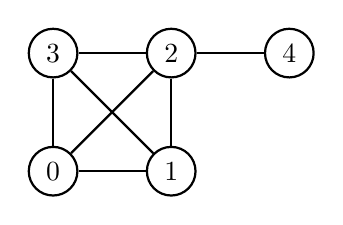
\begin{tikzpicture}[node distance={15mm}, thick, main/.style = {draw, circle}]
				\node[main] (0) {$0$}; 
				\node[main] (1) [right of=0] {$1$}; 
				\node[main] (2) [above of=1] {$2$}; 
				\node[main] (3) [above of=0] {$3$}; 
				\node[main] (4) [right of=2] {$4$};
				\draw (0) -- (1);
				\draw (0) -- (2);
				\draw (0) -- (3);
				\draw (1) -- (2);
				\draw (1) -- (3);
				\draw (2) -- (3);
				\draw (2) -- (4);
			\end{tikzpicture} 
		\end{center}
		
		We want to compute $MH_{2,2}(G)$.
		From Definition \ref{def_MH} we need to evaluate the quotient between the kernel of $\partial_2$ and the image of $\partial_3$.
		So consider the map $\partial_2 : MC_{2,2}(G) \to MC_{1,2}(G)$.
		$MC_{2,2}(G)$ is generated by the $2$-paths (i.e., triplets) in $G$ of length $2$. 
		Therefore, $MC_{2,2}(G)$ is generated by the following $44$ elements: (0, 1, 0), (0, 1, 2), (0, 1, 3), (0, 2, 0), (0, 2, 1), (0, 2, 3), (0, 2, 4), (0, 3, 0), (0, 3, 1), (0, 3, 2), (1, 0, 1), (1, 0, 2), (1, 0, 3), (1, 2, 0), (1, 2, 1), (1, 2, 3), (1, 2, 4), (1, 3, 0), (1, 3, 1), (1, 3, 2), (2, 0, 1), (2, 0, 2), (2, 0, 3), (2, 1, 0), (2, 1, 2), (2, 1, 3), (2, 3, 0), (2, 3, 1), (2, 3, 2), (2, 4, 2), (3, 0, 1), (3, 0, 2), (3, 0, 3), (3, 1, 0), (3, 1, 2), (3, 1, 3), (3, 2, 0), (3, 2, 1), (3, 2, 3), (3, 2, 4), (4, 2, 0), (4, 2, 1), (4, 2, 3), (4, 2, 4).
		
		Similarly, $MC_{1,2}(G)$ is generated by the pairs representing $1$-paths in $G$ of length $2$: (0, 4), (1, 4), (3, 4), (4, 0), (4, 1), (4, 3).
		
		We thus have that the kernel of $\partial_2$ is generated by the $38$ elements whose length diminishes when the middle vertex is removed. That is all elements in $MC_{2,2}(G)$ except (0, 2, 4), (1, 2, 4), (3, 2, 4), (4, 2, 0), (4, 2, 1), (4, 2, 3).  
		
		Being $\partial_2$ a linear operator we can represent it in the following way: we construct the associated matrix indexing the rows and the columns with the elements of $MC_{1,2}(G)$ and $MC_{2,2}(G)$ respectively.
		We then evaluate the differential as stated in Definition \ref{differential} and fill the matrix with the coefficients appearing in the evaluation.
		So for example, $\partial_2 (0,1,2)=0\cdot (0, \hat{1}, 2)=0\cdot (0, 2)$, since $\ell(0,1)<2$, and thus the entry in position $((0,2),(0,1,2))$ will be zero.
		Similarly, $\partial_2 (0,2,4)=1\cdot (0, \hat{2}, 4)=1\cdot (0, 4)$, since $\ell(0,4)=2$, and thus the entry in position $((0,4),(0,2,4))$ will be one.
		
		\begin{figure}
			\hspace{-1cm}
			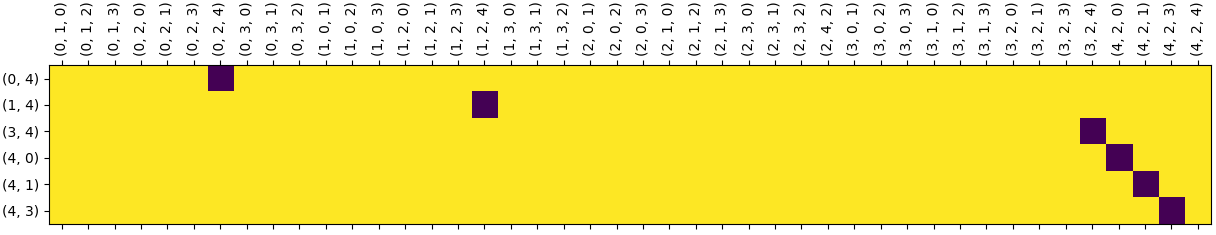
\includegraphics[scale=0.45]{images/kernel_toy_example.png}
			\caption{Matrix representation of $\partial_2$. The $+1$ entries are represented in purple, while the $0$ entries are filled with yellow.}
		\end{figure}
		
		For what concerns the image of $\partial_3$, we need to see which elements of $MC_{3,2}$ are sent to $MC_{2,2}$.
		But since $MC_{3,2}(G)$ is generated by the 4-tuples representing $3$-paths in $G$ of length $2$, and since any path connecting 4 vertices must have length at least 3, $MC_{3,2}(G)$ is the trivial group $\langle 0 \rangle$.
		Therefore the image of $\partial_3$ is $\langle 0 \rangle$.
		In conclusion, we have that 
		\[
		MH_{2,2}(G)=\frac{\ker(\partial_2)}{\imm(\partial_3)}=\ker(\partial_2),
		\]
		and so $|MH_{2,2}(G)|=38$.
	\end{example}
	
	\begin{remark}
		\label{LowerTriangRem}
		We point out that if we represent the ranks of the magnitude homology groups of a graph in a $(k,\ell)$-table as in Table \ref{TableC5}, we will always have that the table is lower triangular.
		In other words, $MH_{k,\ell}(G)\neq 0$ implies that $k \leq \ell$.
		This is because if $MH_{k,\ell}(G)\neq 0$ then $MC_{k,\ell}(G)\neq 0$, and so there is at least a tuple $(x_0,\dots,x_k)$ satisfying $\ell(x_0,\dots,x_k)=d(x_0,x_1)+\cdots+d(x_{k-1},x_k) = \ell$.
		Now, since consecutive vertices are distinct by construction, $d(x_i,x_{i+1})$ is at least $1$ for every $0\leq i\leq k-1$, which means $k$ can be at most $\ell$.
		
		\begin{table}
			\begin{center}
				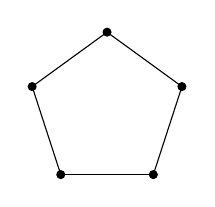
\begin{tikzpicture}[scale=0.5]
					\foreach \x in {0,72,...,288}
					\draw (\x+90:2cm) -- (\x+72+90:2cm);
					\foreach \x in {0,72,...,288}
					\draw [fill](\x+90:2cm) circle (0.1cm);
				\end{tikzpicture}
				\quad
				\begin{tabular}{rr|rrrrrr}
					&&&&&$k$\\
					&&0&1&2&3&4&5\\ 
					\hline                                                               
					& 0 &5\\
					& 1 & &10\\                                          
					& 2 & & &10\\                                          
					$l$& 3 & & &10 &10\\                                          
					& 4 & & &   &30 &10\\                                         
					& 5 & & &   &   &50 &10\\           
				\end{tabular}
			\end{center}
			\caption{Ranks of $MH_{k,l}(C_5)$ computed using Python \textbf{ADD GIT REF}}
			\label{TableC5}
		\end{table}
		
	\end{remark}
	
	It is proven in \cite{hepworth2015categorifying} (Proposition 9) that given a graph $G$, if we indicate by $V$ the set of vertices and by $2E$ the set of oriented edges, then $MH_{0,0}(G)$ is the free abelian group on $V$ and $MH_{1,1}(G)$ is the free abelian group on $2E$.
	
	This provides us with an interpretation of the first two groups on the diagonal, but leaves the question about the meaning of other magnitude homology groups open.
	
	\section{Interpretation of magnitude homology}
	
	The aim of this section is to establish an interpretation for magnitude homology groups on the first and second diagonal.
	
	Our starting point was to reduce the size of the magnitude chain $MC_{k,l}(G)$. 
	In fact, consider for example the group $MC_{2,2}(G)$ of example \ref{toyexample}.
	The generator (0, 1, 0) is the tuple corresponding to the path going twice across the edge (0, 1), and so its presence does not provide any information about the graph and just ``adds noise'' to the information contained in both the magnitude chain and in the magnitude homology group.
	Therefore, we revise the definition of magnitude chain considering the ``plain'' subgroup of $MC_{k,l}(G)$, that is the subgroup of paths where a vertex is never required to be revisited.
	
	\begin{definition}(Plain magnitude chain)
		Let $G$ be a graph.
		We define the plain $(k,l)$-magnitude chain $PMC_{k,l}(G)$ to be the free abelian group generated by tuples $(x_0,\dots,x_k)$ of vertices of $G$ such that $(x_0,\dots,x_k)$ is a $k$-path of length $l$ with $x_i \neq x_j$ for every $0\leq i,j \leq k$.
	\end{definition}
	
	Keeping the same differential as before we can construct the \emph{plain magnitude chain complex} $PMC_{*,l}(G)$
	\[
	\cdots \to PMC_{k+1,l}(G) \xrightarrow{\partial_{k+1}} PMC_{k,l}(G) \xrightarrow{\partial_{k}} PMC_{k-1,l}(G) \to \cdots
	\]
	and subsequently define the \emph{plain (k,l)-magnitude homology group}
	\[
	PMH_{k,l}(G) = H_k(PMC_{*,l}(G)) = \frac{\ker(\partial_k)}{\imm(\partial_{k+1})}.
	\]
	
	\begin{remark}
		\label{PMHsubgroup}
		We point out that all definitions and properties regarding magnitude homology proved in \cite{hepworth2015categorifying} and \cite{leinster2021magnitude} continue to be valid for plain magnitude homology.
		This comes from the fact that, by construction, $PMC_{k,l}(G)$ is a subgroup of $MC_{k,l}(G)$, being generated by a subset of the generating set of the $(k,l)$-magnitude chain, and since we did not change the definition of the differential operator $\partial_k$ it follows that the plain magnitude homology group $PMH_{k,l}(G)$ is a subgroup of the magnitude homology group $MH_{k,l}(G)$ for every $k,l\geq 0$.
		
		In particular, with this new definition, $PMH_{0,0}(G)$ and $PMH_{1,1}(G)$ are still counting the number of vertices and edges in a graph respectively, since the generators of the groups $MC_{0,0}(G)$ and $MC_{1,1}(G)$ already satisfy the condition of not revisiting vertices.
	\end{remark}
	
	%\textbf{Notation.} Since from now on we will make use of the $(k,l)$-plain magnitude chain only, with an abuse of notation we will indicate $PMC_{k,l}(G)$ as just $MC_{k,l}(G)$.
	
	\subsection{First diagonal: counting triangles and squares}
	\label{FirstDiagonal}
	We are concerned in this section with the analysis of the information contained in the groups $PMH_{k,k}(G)$.
	Notice that Remark \ref{LowerTriangRem} implies that $PMC_{k+1,k}(G)$ (and more in general $MC_{k+1,k}(G)$) will always be the trivial group $\langle 0 \rangle$, hence the image of $\partial_{k+1}$ will be $\langle 0 \rangle$, meaning the plain homology group $PMH_{k,k}(G)$ will be entirely determined by $\ker(\partial_k)$.
	
	
	Consider now $PMH_{2,2}(G)=\ker(\partial_2)$.
	Take the matrix associated to $\partial_2$ constructed as described in example \ref{toyexample} and notice the following facts.
	
	\begin{itemize}
		\item The dimension of the kernel of our matrix is equal to the number of all-zero columns plus the number of columns that are ``copies'' of a previously written column.
		\item The number of all-zero columns is (modulo automorphisms) equal to the number of triangles contained in the graph. 
		This is because if a $2$-path $(x_0,x_1,x_2)$ is sent to zero after removing the vertex $x_1$, it means that the shortest path between $x_0$ and $x_2$ has length smaller than $2$. 
		So there exists and edge $(x_0,x_2)$ and equivalently a triangle $(x_0,x_1,x_2)$.
		\item The number of repeated non-zero columns in the kernel indicates how many $2$-paths $(x_0,x,x_2)$ are sent to the same $1$-path $(x_0,x_2)$, and this enables us to produce (at least) an estimate for the number of $4$-cycles contained in the graph.
		Indeed, if $\ell(x_0,x,x_2)$ does not decrease after removing the middle vertex $x$, then this means that any shortest path from $x_0$ to $x_2$ is of length $2$. In other words, two $2$-paths with the same image signify the presence of a $4$-cycle in the graph.
	\end{itemize}
	
	Given this, to obtain the number of $3$-cycles contained in our graph we need to divide the number of all-zero columns by $6$, i.e. by the cardinality of the automorphisms group of the triangle $D_3$.
	
	For what concerns the count of $4$-cycles, notice that the number of non-zero columns will be $2N$ (since we are considering all possible orientations), so we first need to divide this number by two.
	At this point, depending on the complexity of the graph, two situations might arise:
	\begin{itemize}
		\item If we know the image of each $2$-path we are able to compute the exact number of $4$-cycles. Indeed if the same column is repeated $n$ times this means there are $n$ $2$-paths $(x,x_1,y)$, $(x,x_2,y)$,...,$(x,x_n,y)$ sharing the same endpoints, and so they identify $\sum_{i=1}^{n-1} i=\frac{(n-1)n}{2}$ $4$-cycles.
		\item In case we are not aware of the image of each $2$-path, we can still produce upper and lower bounds for number of $4$-cycles contained in our graph.
		Indeed, to produce a square we need at least two $2$-paths $(x,x_1,y)$, $(x,x_2,y)$ with the same image $(x,y)$, so the number of $4$-cycles will be at least $\lfloor \frac{N}{2} \rfloor$.
		Also, the $N$ non-zero columns might all be sharing the same endpoints, in which case the number of $4$-cycles would increase to $\sum_{i=1}^{N-1} i=\frac{(N-1)N}{2}$.
		So, we are able to conclude that the number $S$ of squares contained in our graph $G$ is
		\[
		\left\lfloor \frac{N}{2} \right\rfloor \leq S \leq \frac{(N-1)N}{2}.
		\]
	\end{itemize}
	
	\begin{example}
		\label{toyexample_triangles_squares}
		Consider the following graph $G$
		
		\begin{center}
			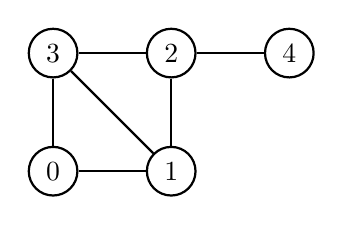
\begin{tikzpicture}[node distance={15mm}, thick, main/.style = {draw, circle}]
				\node[main] (0) {$0$}; 
				\node[main] (1) [right of=0] {$1$}; 
				\node[main] (2) [above of=1] {$2$}; 
				\node[main] (3) [above of=0] {$3$}; 
				\node[main] (4) [right of=2] {$4$};
				\draw (0) -- (1);
				\draw (0) -- (3);
				\draw (1) -- (2);
				\draw (1) -- (3);
				\draw (2) -- (3);
				\draw (2) -- (4);
			\end{tikzpicture} 
		\end{center}
		
		We want to compute $PMH_{2,2}(G)$.
		The plain magnitude chain $PMC_{2,2}(G)$ is generated by (0, 1, 2), (0, 1, 3), (0, 3, 1), (0, 3, 2), (1, 0, 3), (1, 2, 3), (1, 2, 4), (1, 3, 0), (1, 3, 2), (2, 1, 0), (2, 1, 3), (2, 3, 0), (2, 3, 1), (3, 0, 1), (3, 1, 0), (3, 1, 2), (3, 2, 1), (3, 2, 4), (4, 2, 1), (4, 2, 3), while $PMC_{1,2}(G)$ is generated by (0, 2), (1, 4), (2, 0), (3, 4), (4, 1), (4, 3), and the matrix representing our differential is the one displayed in Figure \ref{matrix_toyexample_plain}.
		
		We see that there are twelve all-zero columns, counting the triangles (0, 1, 3, 0) and (1, 2, 3, 1).
		We also have four non-columns, so modulo orientation they are just two and therefore they identify one $4$-cycle.
		In this example they represent the square (0, 1, 2, 3, 0).
		
		\begin{figure}
			\centering
			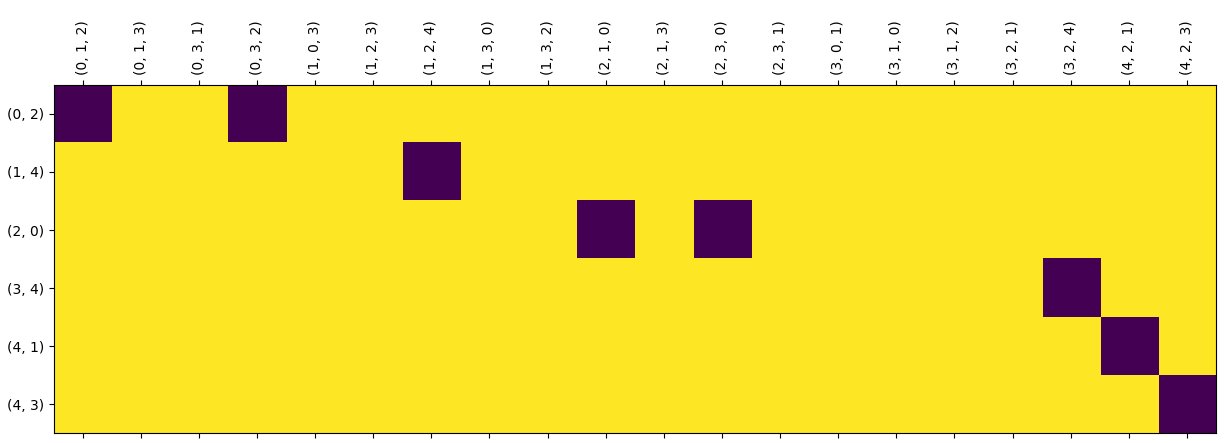
\includegraphics[scale=0.4]{images/kernel_toy_example_plain.png}
			\caption{Matrix representation of $\partial_2:PMC_{2,2}(G) \to PMC_{1,2}(G)$. The $+1$ entries are represented in purple, while the $0$ entries are filled with yellow.}
			\label{matrix_toyexample_plain}
		\end{figure}
		
	\end{example}
	
	
	An analysis on the higher degree magnitude homology groups on the diagonal reveals that the $PMH_{k,k}(G)$'s contain information about which $k$-tuples of vertices of $G$ contain all possible triangles. 
	Indeed, think about all-zero columns in a groups $PMH_{k,k}(G)$, $k \geq 3$.
	If a $(k-1)$-tuple $(x_0,\dots,x_k)$ is sent to zero, this means all the summand maps $\partial_{k,i}$ defining $\partial_k$ have image zero, which in turns indicate that for every $1\leq i \leq k-1$ $\ell(x_0,\dots,x_{i-1},x_{i+1},\dots,x_k)<l$.
	Therefore, for every $1\leq i \leq k-1$ there exists a triangle $(x_{i-1,x_i,x_{}i+1})$, and this provides a hint on where to look for a clique in our graph $G$.
	
	\subsection{Second diagonal: counting 4-cliques and 5,6-``near-cliques''.}
	
	We are concerned in this section with the analysis of the information contained in the groups $PMH_{k-1,k}(G)$.
	
	While the question about a general interpretation for all magnitude homology groups $PMH_{k-1,k}(G)$ on the second diagonal remains open, we were able to understand the information contained in $PMH_{2,3}(G)$.
	Specifically, we believe the third plain magnitude homology group on the second diagonal provides us with information regarding the number of $4$-cliques, $5$-cliques and $6$-cliques in the graph.
	
	Consider the following chain
	\begin{equation*}
		\begin{matrix}
			... &\to & PMC_{3,3}(G)      &\to & PMC_{2,3}(G)            &\to & PMC_{1,3}(G) &\to & 0. \\
			&    & \vin              &    & \vin                    &    & \vin         &    &    \\
			&    & (x_0,x_1,x_2,x_3) &    & (x_0,\hat{x},x_2,x_3) &    & (x_0,\hat{x},\hat{y},x_3) & &
		\end{matrix}
	\end{equation*}
	
	and assume $x_3 \neq \hat{x}$.
	
	If $(x_0,\hat{x_1},x_2,x_3) \in \ker(\partial_2)$ then one of the following is true:
	\begin{itemize}
		\item At least one other different $3$-tuple in $PMC_{2,3}(G)$ is sent to the same $2$-tuple in $PMC_{1,3}(G)$, which means there is either a $4$-cycle or a $6$-cycle.
		\item The considered tuple in $PMC_{2,3}(G)$ is sent to zero, which means there exists either a $4$-cycle or a $5$-cycle.
	\end{itemize}
	
	Now, when we quotient by the image of $\partial_3$ we are in fact disregarding the elements $(x_0,\hat{x_1},x_2,x_3) \in PMC_{2,3}(G)$ such that $\ell(x_0,\hat{x_1},x_2,x_3)=\ell(x_0,x_1,x_2,x_3)$. That is, we are disregarding the tuples that do not contain the triangle $(x_0,x_1,x_2)$, and that therefore cannot be part of a clique.
	
	Summarizing, $PMH_{2,3}(G)$ is counting $4$-cliques and candidates $5,6$-cliques.
	
	\begin{remark}
		We point out that the hypothesis ``$x_3 \neq \hat{x}$'' is crucial to obtain this interpretation. 
		Indeed, without this assumption it could happen that $x_3 = \hat{x}$, which would mean ``revisiting an edge'' and adding a lot of noise to $PMH_{2,3}(G)$.
	\end{remark}
	
	We recall the definition of \emph{diagonal graph} introduced by Hepworth and Willerton in \cite{hepworth2015categorifying}.
	
	\begin{definition}
		A graph $G$ is called diagonal if $MH_{k,l}(G) = 0$ whenever $k \neq l$.
	\end{definition}
	
	The provided interpretation of $PMH_{2,3}(G)$ suggest the following fact.
	
	\begin{proposition}
		If a graph $G$ is diagonal, then it is clique-free.
	\end{proposition}
	
	\begin{proof}
		Suppose G is diagonal, then $MH_{k,l}(G) = 0$ whenever $k \neq l$ and by Remark \ref{PMHsubgroup} $PMH_{k,l}(G)=0$ if $k \neq l$. 
		In particular $PMH_{2,3}(G)=0$, meaning the graph contains no $4$-clique, and therefore no bigger clique.
	\end{proof}
	
	\section{Relation with clustering coefficients}
	
	In Graph Theory, a clustering coefficient is a structural feature that measures the degree to which nodes in a graph tend to cluster together.
	In other words, it tells how connected a vertex’s neighbors are to one another.
	There are two existing versions of this measure.
	The \emph{global}, which was designed by Wasserman and Faust in \cite{wasserman1994social} to give an overall indication of the clustering in the network, and the \emph{local}, first defined by Watts and Strogatz in \cite{watts1998collective} to give an indication about the tendency to cluster near a specific node.
	
	In this section we provide a way to compute both clustering coefficients of a graph $G=(V,E)$ via $PMH_{2,2}(G)$, determining thus a close relation between these tools.
	
	
	\subsection{Local clustering coefficient}
	
	The local clustering coefficient $C_i$ of a node $x_i$ describes the likelihood that the neighbours of $x_i$ are also connected.
	To compute $C_i$ we consider the neighborhood $N_i$ of $x_i$, where $N_i=\{x_j:(x_i,x_j)=e_{ij}\in E\}$ and compute the fraction of the number of links between the vertices within $N_i$ divided by the number of links that could possibly exist between them.
	That is, we set
	\[
	C_i = \frac{2\{e_{jk}:x_j,x_k \in N_i \text{ and } e_{jk}\in E\}}{d_i(d_i -1)},
	\]
	where $d_i=|N_i|$ is the degree of the vertex $x_i$.
	
	In other words, we are dividing the number of triangles $x_i$ is part of by the number of $2$-paths of length $2$ containing $x_i$.
	
	Therefore, call $PMC_{2,2}^i(G)$ the subgroup of $PMC_{2,2}(G)$ such that $x_i$ is the middle vertex of any $2$-path, so $PMC_{2,2}^i(G)=\{(x,x_i,y): \ell(x,x_i,y)=2\}$.
	Then, by section \ref{FirstDiagonal}, the number of triangles containing $x_i$ is precisely the number of all-zero columns of $\ker(\partial_2(PMC_{2,2}^i(G)))$.
	Calling this number $Z_i$, we can write the local clustering coefficient as
	\[
	C_i = \frac{2 Z_i}{d_i(d_i -1)}.
	\]
	
	\begin{remark}
		Given the connection just established between the local clustering coefficient and plain magnitude homology, one could think of using $PMH_{2,2}$ in a network analysis context as a \emph{centrality measure}: if for a given vertex $v_i$ the number $Z_i$ defined above takes low values it means there are few connections between neighbors of $x_i$, meaning $x_i$ has a lot of power over information flow. 
	\end{remark}
	
	
	\subsection{Global clustering coefficient}
	
	The global clustering coefficient $C$ is based on $3$-tuples, i.e. on elements of $PMC_{2,2}$, and is computed as the number of closed $3$-tuples (or $3  \times$ triangles) over the total number of $3$-tuples (both open and closed).
	That is, calling $Z$ the number of all-zero columns in $\ker(\partial_2(PMC_{2,2}(G)))$
	\[
	C = \frac{Z}{|PMC_{2,2}(G)|}.
	\]
	
	\section{Expected value of $PMH$ for Erdos-Renyi graphs}
	
	The aim of this section is to estimate the rank of a plain magnitude homology group of an Erdos-Renyi graph [\textbf{ADD REF}].
	
	Recall that the Erdos-Renyi model was introduced in 1959 by the Hungarian mathematicians after whom it is named, and it is a model for generating random graphs.
	Specifically, in the $G(n,p)$ model a graph on $n$ nodes is constructed by connecting labeled nodes randomly with probability $p$, and each edge is added independently from every other edge. 
	
	\subsection{First diagonal}
	
	We start by focusing on the expectation of ranks of $PMH_{2,2}$.
	From section \ref{FirstDiagonal} we know that the rank of $PMH_{2,2}$ is completely determined by the kernel on $\partial_2$, and that this kernel counts the number of 3-cycles and 4-cycles in the graph.
	
	In the following we will make use of McDiarmid's inequality [\textbf{ADD REF}], which we now recall.
	
	\begin{definition}
		A function $f:X_1 \times X_2 \times \cdots \times X_n \to \R$ is said to satisfy the bounded differences property if substituting the value of the $i$-th coordinate $x_i$ costs at most $c_i$ to the function $f$.
		In other words, if there are constraints $c_1,c_2,\dots,c_n$ such that for every $i \in \{1,\dots,n\}$ it holds
		\[
		\sup_{y_i \in X_i} \left| f(x_1,\dots,x_{i-1},x_i,x_{i+1},\dots,x_n) - f(x_1,\dots,x_{i-1},y_i,x_{i+1},\dots,x_n) \right| \leq c_i.
		\]
	\end{definition}
	
	\begin{definition}[McDiarmid's Inequality]
		Let $f:X_1 \times X_2 \times \cdots \times X_n \to \R$ satisfy the bounded differences property with bounds $c_1,\dots,c_n$.
		Consider independent variables $x_i \in X_i$ for every $i$.
		Then for any $\varepsilon >0$
		\[
		\Prob[\left|f(x_1,x_2,\dots,x_n)-\E[f(x_1,x_2,\dots,x_n)]\right| \geq \varepsilon] \leq 2 \exp \left(-\frac{2\varepsilon^2}{\sum_{i=1}^n c_i^2} \right).
		\]
		
	\end{definition}
	
	Let now $T$ and $S$ denote the number of triangles and squares respectively in $G(n,p)$.
	Then the expected number of triangles $\E(T)$ equals $3 \binom{n}{3}p^3$, and similarly $\E(S)=4 \binom{n}{4}p^4$.
	
	Moreover, the number of triangles is $3n$-Lipschitz with respect to the edges of the graph (meaning that when we change one edge this result in changing at most $3n$ triangles).
	Further, we can give a similar argument and say that the number of squares is $4n$-Lipschitz with respect to the edges of the graph.
	Therefore, for the sake of easing the computation, we will assume both quantities to be $4n$-Lipschitz.  
	
	With these assumption the functions counting then number of triangles and squares in $G(n,p)$ both satisfy the bounded differences property with bounds $c_i = 4n$ for every $i$.
	It is thus possible to write
	\[
	\Prob[\left|T - \E[T]\right|\geq n^{\frac{5}{2}}] \leq  2 \exp \left(-\frac{2n^5}{\binom{n}{2}(4n)^2} \right) \leq 2 \exp \left(-\frac{2n^5}{16 n^2} \frac{2}{n^2} \right) = 2 \exp \left(-\frac{1}{4}n \right),
	\]
	and also
	\[
	\Prob[\left|S - \E[S]\right|\geq n^{\frac{5}{2}}] \leq  2 \exp \left(-\frac{1}{4}n \right).
	\]
	
	As a result, both values of $T$ and $S$ are within $n^{\frac{5}{2}}$ of their expected value with probability $\left(1- 2\exp \left(-\frac{1}{4}n \right) \right)^2 \leq 1-4\exp\left(-\frac{1}{4}n\right)$.
	So $T+S$ satisfies 
	\[
	\left(3 \binom{n}{3}p^3 - n^{\frac{5}{2}}\right) + \left(4 \binom{n}{4}p^4 - n^{\frac{5}{2}}\right)
	\leq T+S \leq
	\left(3 \binom{n}{3}p^3 + n^{\frac{5}{2}}\right) + \left(4 \binom{n}{4}p^4 + n^{\frac{5}{2}}\right)
	\]
	and thus $T+S \sim \frac{(np)^4}{6} + O(n^{-1})$ in these cases.
	The remaining cases influence the expected value by at most $4\exp\left(-\frac{1}{4}n\right)$. 
	Hence we can conclude that
	\[
	T+S = \rank(PMH_{2,2}) \sim \frac{(np)^4}{6} + O(n^{-1}).
	\]
	
	
	\section{Algorithm complexity}
	
	\section{Conclusions}
	
	\bibliographystyle{splncs04}
	\bibliography{bibliography}
	
	\section{Problems to solve}
	
	\begin{enumerate}
		\item The information in the magnitude homology groups $MH_{2,2}$ and $MH_{2,3}$ is "not divided", meaning we are just given the dimension of the kernel without the distinction between all-zero columns and repeated columns.
		\item Add in the software the hypothesis "$x_3 \neq \hat{x_1}$". This is not trivial because the software doesn't really "see" $\hat{x_1}$, it just computes the length of the path supported by the tuple $(x_0,\hat{x_1},x_2,x_3)$.
	\end{enumerate}

\section{Ideas for the future}

\begin{enumerate}
	\item Network analysis:
	\begin{itemize}
		\item Construct a time series using active nodes of a network
		\item Detect small cycles and cliques using MH
		\item Detect persistent structures using PH
	\end{itemize}

	\item Prove that (see if.. but I think so) MH is a stable tool:
	\begin{itemize}
		\item Define an "interaction index" which should be a measure the tendency of a general vertex $v$ to interact with other vertices in the graph (maybe taking inspiration from connectivity index [ADD RED] and cycle index [ADD RED]). Maybe the global clustering coefficient can be used?
		\item Define a distance between two graphs $G$ and $G'$ using the interaction index
		\item See if a small variation in the interaction implies a small variation in MH
		\item Maybe define a "MH diagram" following the idea of persistence diagrams and do the above point for this MH diagram  
	\end{itemize}
	
\end{enumerate}

	
\bibliographystyle{unsrt}
\bibliography{bibliography}

\end{document}